\documentclass[10pt,a4paper]{article}
\usepackage{graphicx,float}

\title{\LARGE
    Project Phase 1: A Detailed Analysis of SUPERCOP on the Dragonboard APQ8060.
}

\author{\large
{\bf Kevin Burns, Robert Lyerly, Reese Moore, Philip Kobezak}\\ 
Virginia Polytechnic Institute \& State University\\
1185 Perry Street, Blacksburg VA\\
\vspace{8mm}
\{kevinpb, rlyerly, ram, pkobezak\}$@$vt.edu\\
}
\date{}

\begin{document}

\maketitle


% INTRODUCTION   
%--------------
% Contains:
%   - a brief overview of the APQ8060 architecture.
%   - how we approached the problem
%   - how we partitioned the tasks
%   - how we automated the profiling
\section{Introduction}
Computers are a ubiquitous part of our society.  As computers become increasingly connected, more of our daily lives are becoming digitized.  As such, it is important that we find new ways to ensure security and privacy.  The field of Cryptography involves designing algorithms and protocols as a means of ensuring services interact with each other in a secure, private way.  Traditionally, cryptographic theory was used to develop algorithms that were highly efficient and very secure on large desktop CPUs.  However, with the dawn of mobile computing there is an increased need for power-aware cryptography.  Research in this field seeks to strike a balance, searching for algorithms that can be used in low-power settings while still being strong and secure.  New cryptographic algorithms must be evaluated on a wide variety of hardware platforms to understand how they perform in practice.

Hash functions play an important part in cryptography.  They are heavily used for authentication and digital signing, two components of cryptography that are necessary for information security.  Designing a good hash function is a complex task - the algorithm must have several characteristics such as uniformity, efficiency and infeasability of reversing the hash.  The National Institute of Standards and Technology (NIST) is responsible for maintaining many cryptographic algorithms, including hash functions.  NIST recently held a competition to generate an alternative to SHA-1 and MD5 because of known attacks for these hash functions.  Many different researchers submitted implementations to the competitions, and the Keccak algorithm was chosen as the official implementation for SHA-3 on October 2, 2012.  However, the software hosted at http://bench.cr.yp.to contains all the SHA-3 implementations submitted to NIST so that anybody may test them.  In the first phase of our project, we were tasked with benchmarking these submissions.

\subsection{Hardware Overview}
Our platform for the first phase of the project was a Snapdragon S3 APQ8060-based Dragonboard, used for prototyping and developing for the Android platform (hereafter referred to as ``the Dragonboard'').  The Dragonboard implements a complete wireless phone system, including a wireless RF card, a sensor card (with accelerometer and gyroscope) and a touchscreen.  The Snapdragon S3 APQ8060 contains several cores for computation and processing:

\begin{enumerate}
	\item ARM1136J-S 384 MHz embedded microprocessor
	\item Qualcomm dual-core Scorpion microprocessor (up to 1.7 GHz), which has the ARM NEON SIMD extensions
	\item Qualcomm QDSP6000 and QDSP4000 DSP cores
	\item ARM7 resource and power management microprocessor
	\item Adreno 220 GPU
\end{enumerate}

Most compute-intensive tasks are run on the larger Scorpion cores (which are designated as ``application cores''), the QDSP6000 DSP and the Adreno 220 GPU.  The ARMv7 instruction set architecture (ISA) is the 7th-generation of the ARM ISA.  It is a RISC ISA and contains a standardized 3-stage pipeline (although implementations may contain longer pipelines) and 16 x 32-bit registers.  ARMv7 also defines the NEON SIMD extensions which specify the interface to a 128-bit SIMD core with an independent pipeline and register file.  It can perform basic arithmetic and logic operations on varying size data types, including signed/unsigned 8-bit, 16-bit, 32-bit or 64-bit words.  The QDSP6000 (or ``Hexagon'') DSP is a programmable DSP designed for application use.  It has several features which make it a flexible platform, including symmetric multi-processing and VLIW/SIMD instructions (in fact, Linux has been ported to run on the Hexagon).  The Adreno 220 GPU is used for 2D and 3D rendering on Android.  It implements several graphic APIs and can be used concurrently by several of the other cores for interleaving CPU, DSP and graphics operations.

\subsection{Problem Statement}
The objective of the first phase of the project was to do a detailed perfomance profiling for a set of hash algorithms provided by the SUPERCOP testsuite. The analyses should try to determine why each algorithm implementation excelled, compared to other implementations,  on the target platform (Dragonboard APQ8060).   

\subsection{Partitioning}
\subsection{Profiling}



% ALGORITHMS
%------------
% Each subsection will contain:
%   - a figure containg the graph of the performance
%   - an analysis of the graph
\section{Algorithms}
\subsection{blake32}
The BLAKE hash function is based on the ChaCha stream cipher, with an additional XOR each round. The way it works is,
the ChaCha algorithm works with a 4 by 4 array of words. BLAKE combines an 8-word hash value with 16 words from the 
message repeatedly, in turn truncating the ChaCha result to obtain the next hash value.The BLAKE hash function has two variants, 
a variant with a word size of 32 bits and a variant with a word size of 64 bits. The first two hash functions we evaluate, blake32 and blake256, are 
of the 32 bit word variety.

\begin{figure}[H]
    \begin{center}
        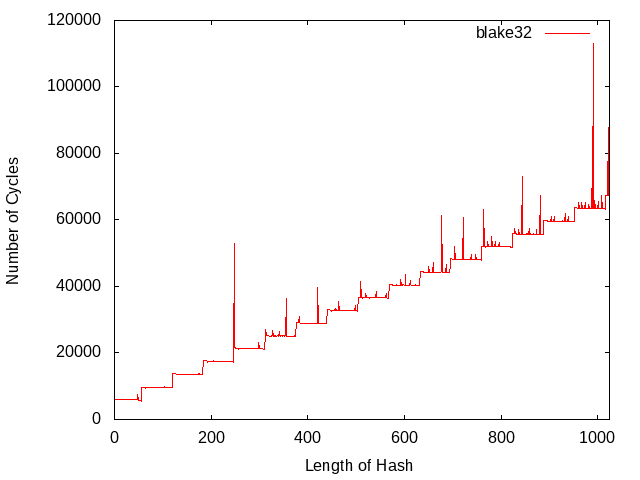
\includegraphics[scale=0.5]{images/blake32.png} 
        \caption{BLAKE with 32-bit words, 10 rounds, and 256-bit output}
    \end{center}
\end{figure}

From the graph above we see that there is a stepwise characteristic. The steps seem to increment every time the hash is divisible by 64. 
This characteristic is present due to the fact that during each iteration 2 words are taken from the message at one time. So a total of 64 bits
of the actual message is processed. This happens 8 times a round, therefore 512-bits are processed per round. So, as our hash size increases by 
multiples of 64 bytes we will see more and more iterations having to be processed.

\subsection{blake256}
    \begin{figure}[H]
        \begin{center}
            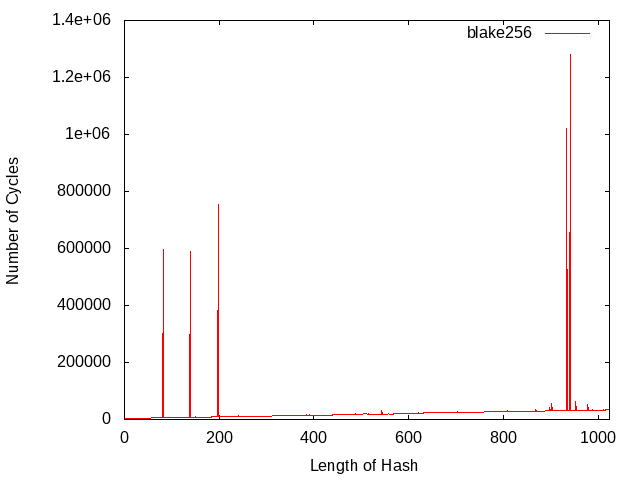
\includegraphics[scale=0.5]{images/blake256.png} 
            \caption{BLAKE with 32-bit words, 14 rounds, and 256-bit output}
        \end{center}
    \end{figure}

The graph above shows a very similar pattern to the blake32 graph. The reason is that blake256 also uses a 32 bit word size. The difference we
see between the blake32 and this graph is the number of cycles. When analyzing the data I found that the cycles per byte for blake32 was twice
that of blake256. This seems counter intuitive as blake256 has an additional 4 rounds to compute each iteration. I speculate that this is
due to the compiler options chosen by the script we ran to find the fastest implementation of each algorithm. The options chosen for blake256 were 
(compiler gcc -mcpu=arm1136jf-s -O -fomit-frame-pointer -fno-schedule-insns 4.4.5) versus the options for blake32 
(gcc -mcpu=arm9tdmi -O2 -fomit-frame-pointer 4.4.5). As we can see the architecture chosen by the script is not the target architecture and could
lead to a number of mis-optimizations. 

\subsection{blake64}
    \begin{figure}[H]
        \begin{center}
            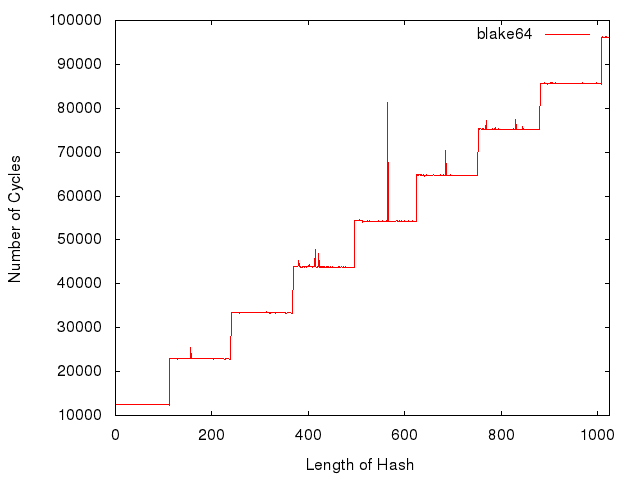
\includegraphics[scale=0.5]{images/blake64.png} 
            \caption{BLAKE with 64-bit words, 14 rounds, and 512-bit output }
        \end{center}
    \end{figure}

The blake64 hashing function increases the word size to 64 bits. Since nothing else changes we see that the widths of each step in our 
stepwise graph is doubled, so 1024 bits long. The cycles per byte were higher than that of the 32-bit word sizes. This is due to the 
fact that the target processor is a 32 bit architecture and does therefore doesn't have a chance to utilize 64 bit words. 

\subsection{blake512}
    \begin{figure}[H]
        \begin{center}
            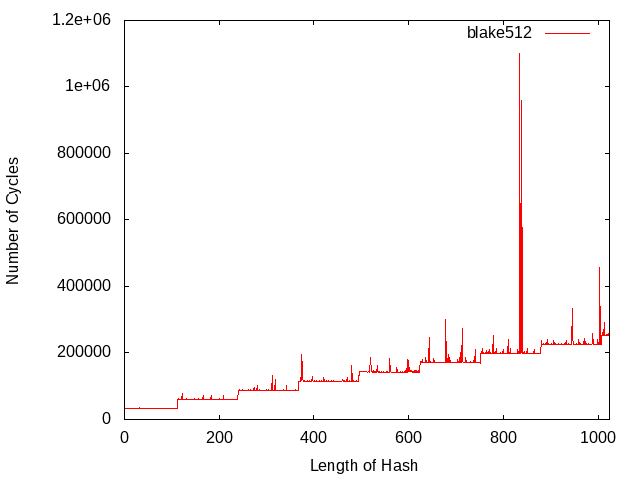
\includegraphics[scale=0.5]{images/blake512.png} 
            \caption{BLAKE with 64-bit words, 16 rounds, and 512-bit output}
        \end{center}
    \end{figure}
The difference between blake512 and blake64 is the number of rounds. This would explain the identical step width, 128 bytes, along with the increase
in cycles for blake512. 

\subsection{cubehash816}
I won't explain the details of cubehash here. I will instead talk about how the choice of variable sizes in the cube hash equation is reflected on the graph, along with the possible influence from the architecture. If we represent the equation as CubeHashi+r/b+f–h(m). Where i is the number of initialization rounds, r is the number of rounds per message block, b is the length of the blocks taken from the message, f is the number finalization rounds, h is the number of output bits, and m is the message. We're given that r is 8 rounds per block, b is 16 bytes in a block, and h is 512 bits of output.
    \begin{figure}[H]
        \begin{center}
            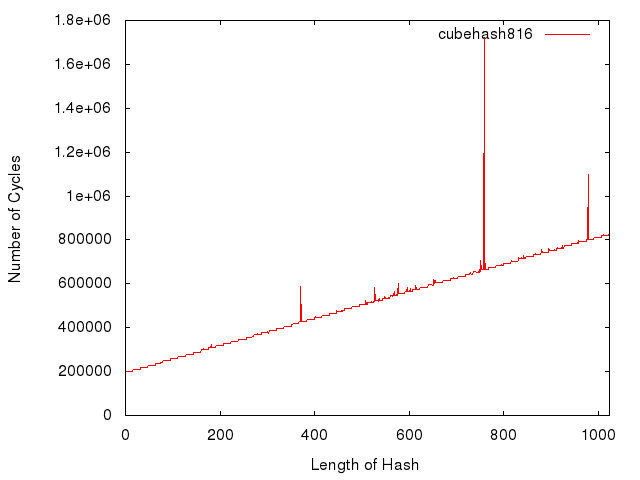
\includegraphics[scale=0.5]{images/cubehash816.png} 
            \caption{CubeHash8/16 with 512-bit output}
        \end{center}
    \end{figure}
It is a little hard to see in the above graph, but it takes on a similar shape to the graphs found in the blake algorithms. That is, it is as step like characteristics. The length of each step is 16 bytes, 128 bits. This appears to be from the size of the blocks processed each round. Each block is 16 bytes as described above. When the message increments by a multiple of 16 we see a rise in the step. As that's one more block that needs to be processed.  
Our target platform can provide 16, 32bit registers for the processing each block. This may be a responsible for the given speed.

\subsection{groestl256}
The groestl algorithm is another block cipher that is based from AES. This function works with l-bit blocks where l is 2n and n is the number of output bits. In this case n is 256 as denoted in the name. 
    \begin{figure}[H]
        \begin{center}
            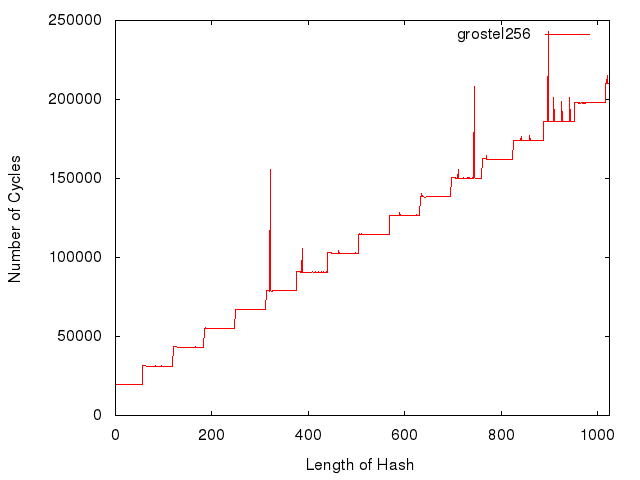
\includegraphics[scale=0.5]{images/grostel256.png} 
            \caption{Grøstl with 256-bit output}
        \end{center}
    \end{figure}
The graph above also shares the step like characteristics of the other graphs. Each step for this plot is 64 bytes, 512 bits in length. From what we know about groestl, it works with l-bit blocks, where we derived above l is 512 bits. We can then correlate this to the nature of the step size witnessed in the graph above.


\subsection{groestl512}
\subsection{jh224}
\subsection{jh256}
\subsection{jh384}
\subsection{jh512}
\subsection{keccak}
\subsection{keccakc1024}
\subsection{keccakc256}
\subsection{keccakc448}
\subsection{keccakc512}
\subsection{keccakc768}
\subsection{md5}


\subsection{mgr{\o}stl256}
The modified-Gr{\o}stl (mgr{\o}stl) algorithm is a modification of the Gr{\o}stl hash algorithm chosen as one of the five finalists of the SHA-3 competition.  Similar to other hash algorithms, an arbitrary length input is padded so that it can be divided into 1024-bit blocks.  The algorithm works by performing a compression function on each block; the compression function involves additions and permutations that reduces the 1024-bit input to a 512-bit intermediate hash.  The output from each of these compression operations serves as input to the next block with a final reduction that shrinks the message to a digest size of 256 bits. 

    \begin{figure}[H]
        \begin{center}
            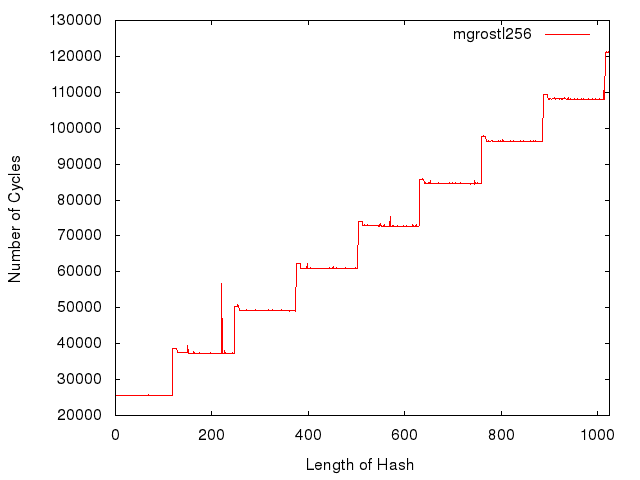
\includegraphics[scale=0.5]{images/mgrostl256.png} 
            \caption{Modifided-Gr{\o}stl with 256-bit output}
        \end{center}
    \end{figure}

\subsection{sha256}
The sha256 and sha512 algorithms are specific implementations of the previous generation SHA-2 hash function defined by NIST.  After effective attacks were found on SHA-1, NIST moved to a better hash algorithm, one which features several improvements (including fewer collisions and no known effective attacks).  Four variants of the algorithms were standardized based on the number of bits produced in the digest (including 256 and 512 bits for sha256 and sha512, respectively).

    \begin{figure}[H]
        \begin{center}
            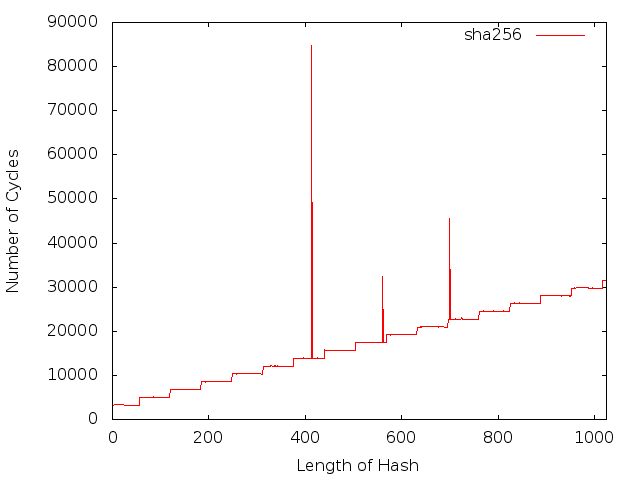
\includegraphics[scale=0.5]{images/sha256.png} 
            \caption{SHA-2 with 256-bit output}
        \end{center}
    \end{figure}

The first algorithm, sha256, works by chopping a message into 512-bit blocks and hashing each block down to 256-bits before continuing on to the next.  The result of entire hash function is added together with the original hash value, producing the final digest.  As is evident from the graph, performance models a step function with a step size of 64 bytes.  The number of blocks needed to represent the message is $\lceil$message length$/ 64 \rceil$ (this converts the number of block into an integer multiple of 64).  As soon as the message requires a higher multiple of 64 bytes, the algorithm must process another block of data.  Therefore, for every additional 64 bytes of data, another additional 64 rounds of SHA-2 must be performed.

\subsection{sha512}

    \begin{figure}[H]
        \begin{center}
            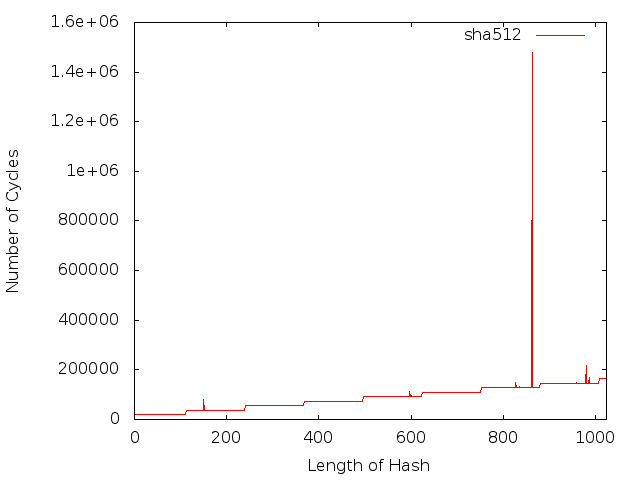
\includegraphics[scale=0.5]{images/sha512.png} 
            \caption{SHA-2 with 512-bit output}
        \end{center}
    \end{figure}

The second SHA-2 algorithm benchmarked, sha512, again produces a step function; closer inspection reveals this graph has slightly different characteristics than the one produced by running sha256.  There are some fundamental changes in the underlying algorithm - first, the digest length is 512-bits and the block size is 1024 bits.  This means that for every additional 128 bytes needed to represent the message, the algorithm must process an extra block of data - hence the step size of 128 bytes.  Because this block length is longer the algorithm must perform more calculations per round, leading to a higher cycles per byte.  Additionally, sha512 performs 80 rounds versus the 64 performed by sha256, leading to another increase in cycle count.

\subsection{skein256256}
The Skein family of hash functions were submitted to the competition by a varied group of individuals and was one of the five finalists for SHA-3.  The Skein hash functions are based on a tweakable block cipher, named the Threefish block cipher.  The Threefish block cipher favors more rounds versus higher complexity; it only performs XOR, addition and shift operations.  It uses keys (which are the same length as the block) and a 128-bit tweak value to generate the key schedule.  These generated keys are then injected every couple of round of the "Mix" operation (XOR, addition, shift); this entire sequence constitutes one round, with the Skein hash performing varying number of such rounds depending on the block size.  One final feature of the Skein family of hash functions is the ability to have arbitrary length outputs, implemented using UBI chaining mode.  Because these hash functions work on 64-bit words, it is not well-suited to the 32-bit architecture of the Scorpion processors.  However, the ARM NEON SIMD instructions can be used to perform many of the round calculations to speed up computation.

    \begin{figure}[H]
        \begin{center}
            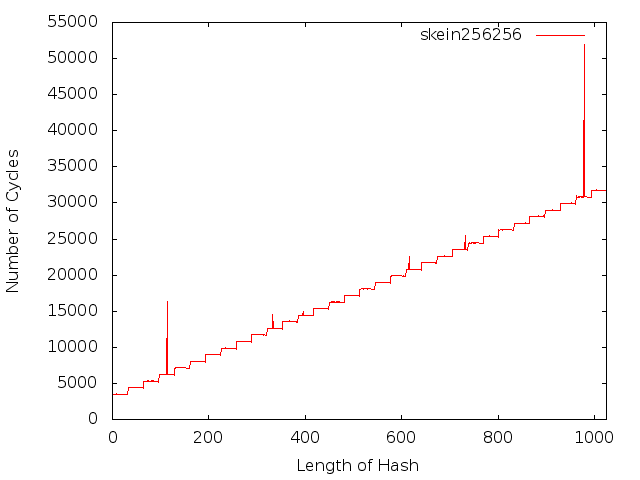
\includegraphics[scale=0.5]{images/skein256256.png} 
            \caption{Skein-256 with 256-bit output}
        \end{center}
    \end{figure}

This instance of the Skein hash function has a block size of 256-bits (32 bytes) and produces a 256-bit digest.  In this instance, the block cipher operates on 32 byte blocks; naturally, with every higher multiple of 32 a new block must be processed, leading the to the step function represented in the graph.  Because the block size is smaller, there are fewer calculations for the block cipher, resulting in shorter runtimes in comparison to the other Skein hash functions.

\subsection{skein512256}

    \begin{figure}[H]
        \begin{center}
            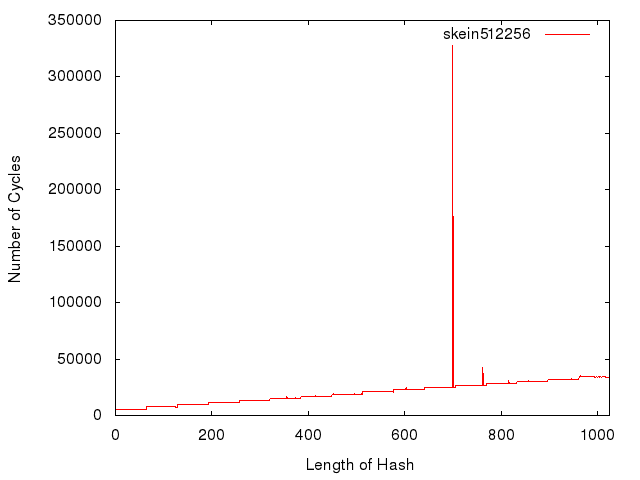
\includegraphics[scale=0.5]{images/skein512256.png} 
            \caption{Skein-512 with 256-bit output}
        \end{center}
    \end{figure}

This instance of the Skein hash function has a block size of 512-bits (64 bytes) and produces a 256-bit digest.  Again, because the block size is 64 bytes, every higher multiple of 64 bytes creates an extra block which must be processed, similar to the previous Skein functions.  The performance of skein512256 is very comparable to the performance of skein256256.  This is because although there are twice as many operations per block in skein512256 (it must handle 64 bytes instead of 32) but there are half as many blocks to process, hence a comparable number of operations must be performed for each algorithm.  The step function is more coarse-grained than skein256256 because of the word size.

\subsection{skein512512}

    \begin{figure}[H]
        \begin{center}
            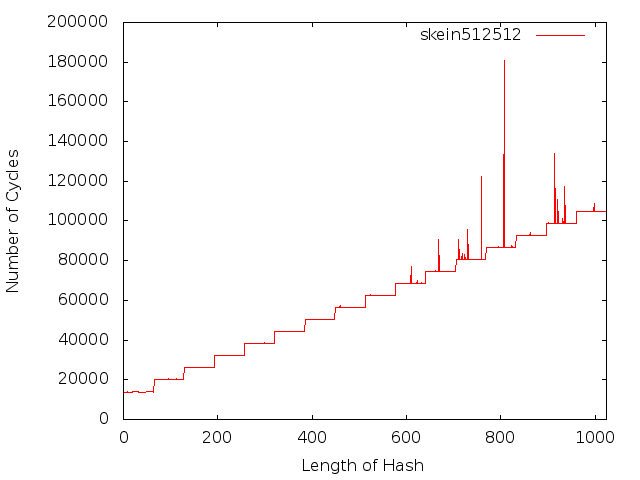
\includegraphics[scale=0.5]{images/skein512512.png} 
            \caption{Skein-512 with 512-bit output}
        \end{center}
    \end{figure}

This instance of the Skein hash function has a block size of 512-bits (64 bytes) and produces a 512-bit digest.  Similar to the other Skein hash funcions, the step size is dictated by the block size; its length is 64 bytes because this instance of the Skein hash function works on 64 byte blocks.  This algorithm shows perfomance slower than skein512256, however - this is because of the output length of the hash.  Skein hash functions use Unique Block Iteration (UBI) chaining to produce the variable size output.  Part of this chaining involves XOR'ing message blocks together with blocks run through the Threefish cipher, and using that output as the input to the next block's chaining.  Because a skein512512 must XOR more words together when chaining the blocks (because the block size is larger), UBI chaining causes performance penalties in comparison to skein512256.

\subsection{skein10241024}
    \begin{figure}[H]
        \begin{center}
            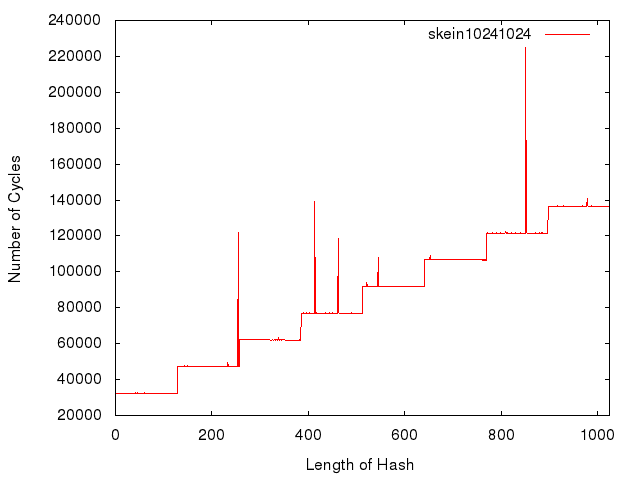
\includegraphics[scale=0.5]{images/skein10241024.png} 
            \caption{Skein-1024 with 1024-bit output}
        \end{center}
    \end{figure}

This instance of the Skein hash function has internal state size of 1024-bits (128 bytes) and produes a 1024-bit digest.  Because the Threefish block cipher works on 128 byte blocks, the step function has a step size of 128 bytes; that is, the number of blocks that must be processed increases with every higher multiple of 128.  Following the analysis for skein512512, this algorithm must also pay a performance penalty for the UBI chaining; it must XOR more words together for each block.  Finally, this implementation has more rounds than other Skein hash functions (80 rounds instead of 72).  Therefore, this implementation has the worst performance of any of the Skein has functions on this architecture.

% CONCLUSION   
%------------
% Contains:
%   - any overall conclusion we can draw from the results of ALL the graphs
%   - lessons learned
\section*{Conclusions}
\end{document}
